\chapter{Generazione di traffico con diversa variabilit\`a}

\section{Distribuzioni di traffico considerate}

Le distribuzioni secondo le quali il traffico si presenta all'ingresso del sistema influenzano in modo marcato le dinamiche che a regime vengono a determinarsi all'interno dello stesso. Per questo motivo \`e di grande importanza osservare la risposta specifica del sistema ad input differenziati, al fine di valutarne le caratteristiche e di meglio comprendere le specifiche peculiarit\`a delle varie distribuzioni in analisi.

Le tipologie di distribuzione prese in considerazione sono, come da specifica:
\begin{itemize}
\item Deterministica 
\item Poissoniana (Exponential)
\item Switched Poisson Process (SPP) 
\item Pareto
\end{itemize}

Il simulatore permette, in funzione del tipo di distribuzione selezionata e dei parametri imposti, di valutare valore medio, varianza ed indice di dispersione relativi al traffico generato.

\begin{figure}[!h]{
	\begin{center}
	   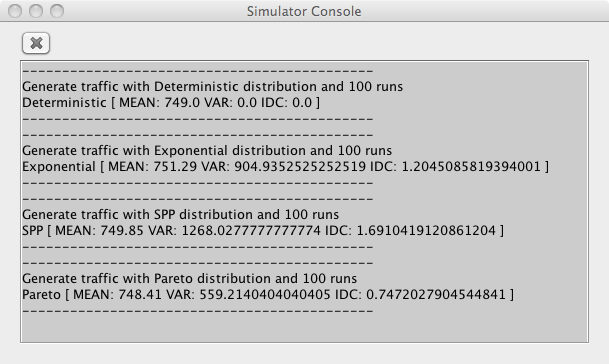
\includegraphics[width=\textwidth]{figures/simconsole.png}
	\end{center}}
	\caption{Esito della simulazione di varie tipologie di traffico (console)}
	\label{fig:console}
\end{figure}


Al termine della computazione, i risultati numerici vengono riportati sulla console appositamente realizzata (fig. \ref{fig:console}).


\subsection{Analisi tecnica}

L'esecuzione della simulazione avviene, analogamente a quanto visto nel capitolo precedente, facendo ricorso alla classe {\tt SimulationRunners}. L'organizzazione gerarchica delle distribuzioni, ottenuta mediante varie specializzazioni della classe {\tt Distribution} rende possibile una gestione trasparente rispetto alla scelta effettuata dall'utente.

Per la gestione della console di sistema, all'interno della quale vengono presentati i risultati delle simulazioni, si \`e ricorsi alla libreria LOG4J\footnote{LOG4J - http://logging.apache.org/log4j/1.2/}
In particolare si \`e realizzata una console su finestra indipendente la cui visualizzazione pu\`o essere (dis)abilitata dall'utente, senza che i dati in essa contenuti vadano persi.

\begin{figure}[!h]{
	\begin{center}
	   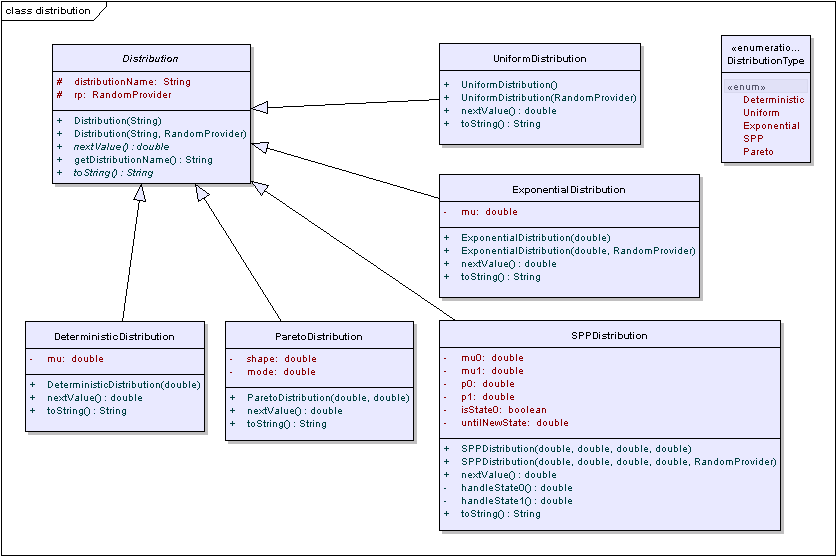
\includegraphics[width=\textwidth]{figures/distributionclass.png}
	\end{center}}
	\caption{Struttura del package {\tt simulator.distribution}}
	\label{fig:distuml}
\end{figure}

La generazione di valori da parte delle classi che implementano la classe astratta {\tt Distribution} (si veda lo schema in fig \ref{fig:distuml}) avviene attraverso il metodo {\tt nextDouble()}, in particolare ogni estensione della classe implementa una spefica funzione in base al tipo di distribuzione rappresentato.

Infine, \`e interessante notare come attraverso il ricorso alla classe {\tt Executor- Service} l'onere computazionale sia stato scisso dalla gestione dell'interfaccia grafica, permettendo cos\`i un'esperienza d'utilizzo esente da blocchi dovuti alla computazione.

%ACHTUNG: su ExecutorService (sopra) si "forza" un acapo manuale, brutto brutto brutto!

%\subsubsection{Nota}
%Per la simulazione di traffico con diversa variabilit\`a trattata in questo capitolo, e per le successive, si \`e fatto affidamento sulla classe {\tt Random} descritta in sezione \ref{sec:rndjava}, date l'ottima efficienza computazionale dello stesso e la scarsa incisivit\`a dei difetti comuni ai generatori lineari congruenziali in genere per l'applicazione in oggetto.
